\chapter{Transactions}
	\section{Definition}
		\begin{itemize}
			\item Transaction resembles flow $($cash, goods, etc.$)$
			\item Transactions are the reason for business in the first place
			\item Application systems must support transaction programs!
			\item \color{red}"Transactions are the heart of economy"\color{black}
		\end{itemize}
			
	
	\section{Concept}
		\begin{itemize}
			\item A transaction is a process, that accesses and may updates data items
				\subitem databases 
				\subitem resource managers
			\item A transaction must see a consistent database at start
			\item During transaction, a database may enter a inconsistent state
			\item After the transaction is done, the Database must be consistent again
			\item There are 2 possible issues:
			\subitem Recovery $($ system crashes and similar $)$ 
			\subitem Concurrency Control $($ keeping the data consistent while multiple transactions are executed $)$
		\end{itemize}
	
	\newpage
	\section{Concurrent Executions}
		\begin{figure}[h!]
			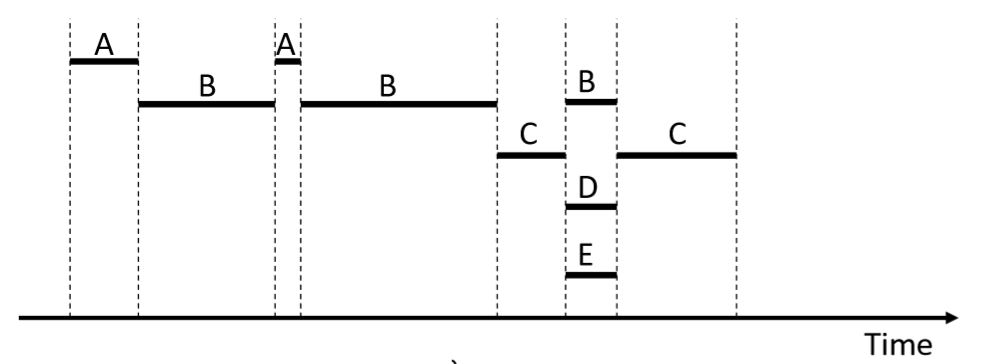
\includegraphics[scale=0.5]{res/Concurrent-Transactions.jpg}
			\caption{Types of Concurrent Transactions}
		\end{figure}
		\begin{itemize}
			\item A,B,C: Interleaved
			\item B,D,E: Simultaneous
			\item all: Parallel Transactions			
		\end{itemize}
	
	\section{Benefits of Concurrency}
		\begin{itemize}
			\item Higher Throughput
			\item More Utilization of the CPU = better value
			\item faster Response Time
		\end{itemize}
		
	\section{Possible Failures}
		\begin{itemize}
			\item System crash
			\item Transaktion Error
			\item Concurrency Control Enforcements $($Scheduler aborts$)$
			\item Disk Failure $($Data lost$)$
			\item Physikal Problems $($wrong Disk hooked up, Fire etc.$)$ 
		\end{itemize}
		
	
	\section{Transaction Processing}
		Transaction Processing is about:
		\begin{itemize}
			\item Maximum throughput
			\item Maximum utilization
			\item Maximum availability 
			\item Maximum scalability
			\item Minimum downtime
		\end{itemize}
	
	\section{ACID}
		\begin{itemize}
			\item Atomicity
				\subitem Transactions are fully reflected in the Resource Manager or are not reflected
			\item Consistency
				\subitem The Consistency of the resources is not harmed by any Transaction
			\item Isolation
				\subitem Transactions made at the same Time, don't need to know from each other to achieve correctnes
			\item Durability
				\subitem If a transaction is completed succesfully, all changes are permanent
		\end{itemize}
	
	\section{Transaction Operations}
	
		\subsection{BOT = Begin of Transaction}
		
			\subsubsection{Implicit BOT}
			
				 Automatically issued on behalf of transaction of first resource manager request (after former EOT) 
				
			\subsubsection{Explicit BOT}
			
				Issuing a BEGIN operation
		
		\subsection{EOT = End of Transaction}
		
			\subsubsection{Implicit EOT}
			
				Resource manager decision based on transaction’s state
				
				\begin{itemize}
					\item May be COMMIT or ABORT
				\end{itemize}
		
			\subsubsection{Explicit EOT}
		
		\subsection{COMMIT}
			Request to make all changes permanent
		
		\subsection{ABORT/Roll back}
			All changes must be reverted
		
	\section{Example in RL}
		\begin{figure}[h!]
			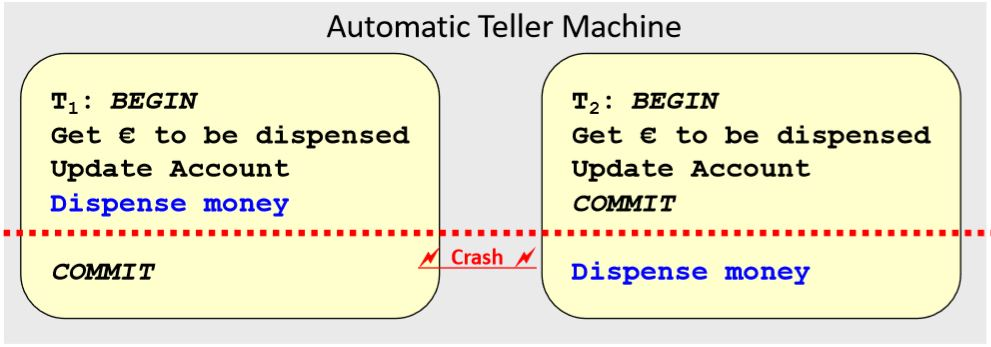
\includegraphics[scale=0.5]{res/real-life-transaction.jpg}
			\caption{Real World Actions In Transactions}
		\end{figure}
	
	\section{Transaction States}
		\begin{itemize}
			\item active
				\subitem  the initial state; the transaction stays in this state while it is executing 
			\item done
				\subitem all statements have been executed
			\item failed 
				\subitem n
			\item aborted normal execution can no longer be achieved
			\item commited
				\subitem after successful completion
			\item aborted
				\subitem transaction was aborted and all changes are reverted
		\end{itemize}
			
		\begin{figure}[h!]
			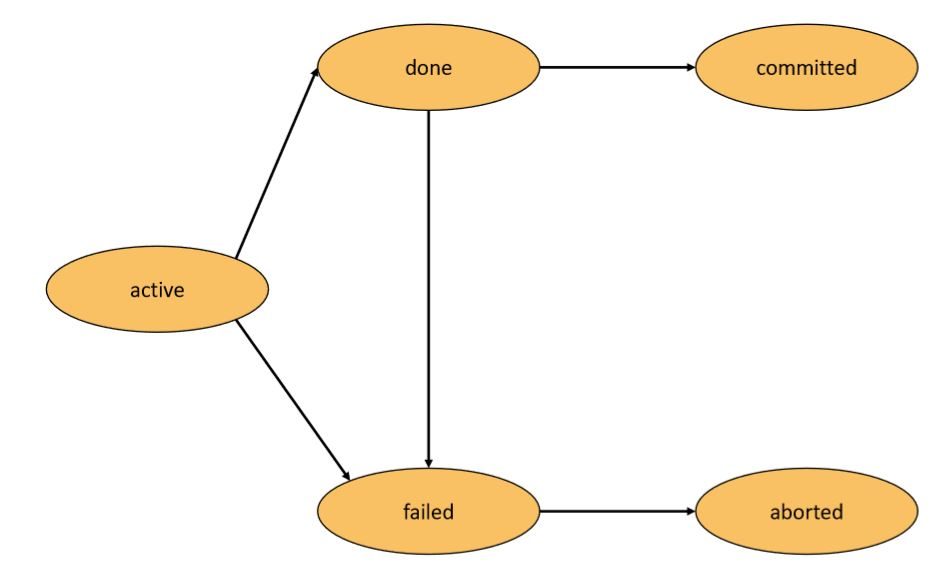
\includegraphics[scale=0.5]{res/state-diagram-transaction.jpg}
			\caption{Transaction State Diagram}
		\end{figure}
	
	\section{Serializability}
		
		\subsection{Schedule}
		
			Order sequence in which concurrent transactions are executed
		
		\subsection{Conflicts}
		
			A conflict occures if and only if two instructions both acces the same data at the same time and at least one of them is a write.\\
			Intuitively, a conflict between i$ _k $ and i$ _j $ forces a (logical) temporal order between them. 
		
		\subsection{Swaps}
		
			If two transactions operate on different data, or don't interfere in general, they can be swaped $ ( $change their order$ ) $ without changing the result.
		
		\subsection{Conflict Serializability}
			
			If a schedule S can be transformed into a schedule S’ by a series of swaps of non-conflicting instructions, we say that S and S’ are \textbf{conflict equivalent} :S $ \equiv $ S’ 
			\begin{figure}[h!]
				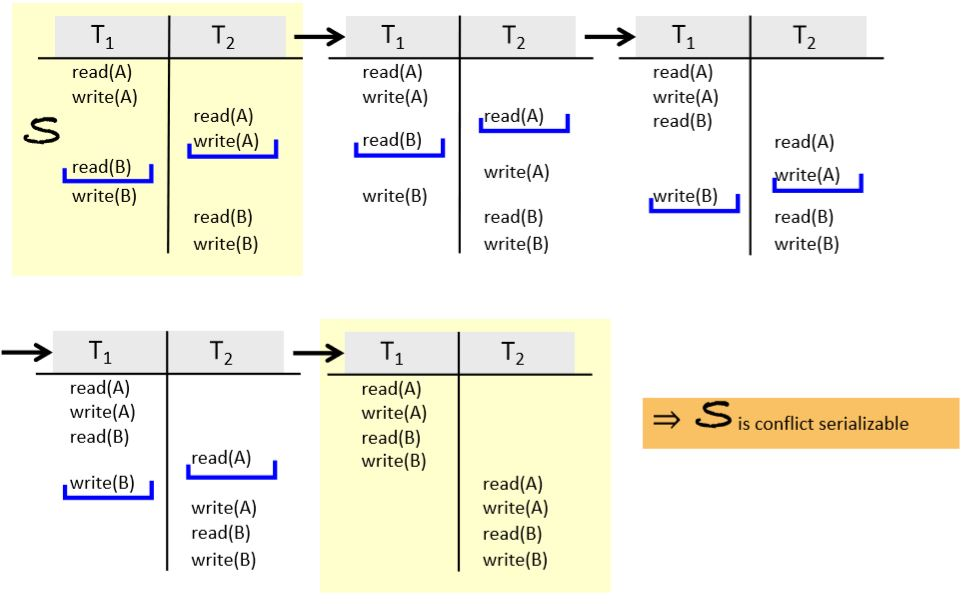
\includegraphics[scale=0.5]{res/conflict_serializable.jpg}
				\caption{Conflict Serializability Example}
			\end{figure}
			
		\subsection{Recoverability}
			Writer must commit before reader, so if the writer aborts, the transaction that read the uncommited changes can and must abort too.\\
			Can lead to cascading aborts what leads to reverting a significant amount of changes
		\subsection{ACA Schedules}
			\begin{itemize}
				\item prevents cascading aborts
				\item For each pair of transactions $ T_{writer} $ and $ T_{reader} $ such that $ T_{reader} $ reads a data item previously written by $ T_{writer} $, the commit operation of the writing  transaction $ T_{writer} $ appears before the readoperation of $ T_{reader} $ 
			\end{itemize}
		\subsection{Testing for Serializability -- Precedence graph}
			transactions = nodes \\
			conflicts = arcs between nodes\\
			accessed item $ ( $that is causing conflict$) $ = label of arc\\
			
			\begin{figure}[h!]
				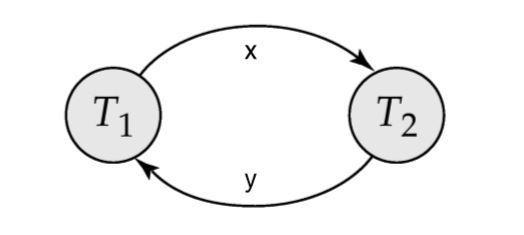
\includegraphics[scale=0.5]{res/precedence_graph_serializable.jpg}
				\caption{Precedence Graph}
			\end{figure}

		Theorem: A schedule is conflict serializable if and only if its precedence graph is acyclic\\
		\\
		Theorem: If precedence graph is acyclic, a serializability order can be obtained by a topological sorting of the graph
		
		
	\newpage	
	\section{Distributed Transactions}
	
		\subsection{Atomicity in distributed transactions}
			If one System loses update, so it cannot commit the transaction when it recovers $ \Rightarrow $ Whole transaction must fail!
		\subsection{Transaction models}
			\subsubsection{X/Open Model}
			
			\subsubsection{Two-phase commit protocol (2PC)}
				\begin{figure}[h!]
					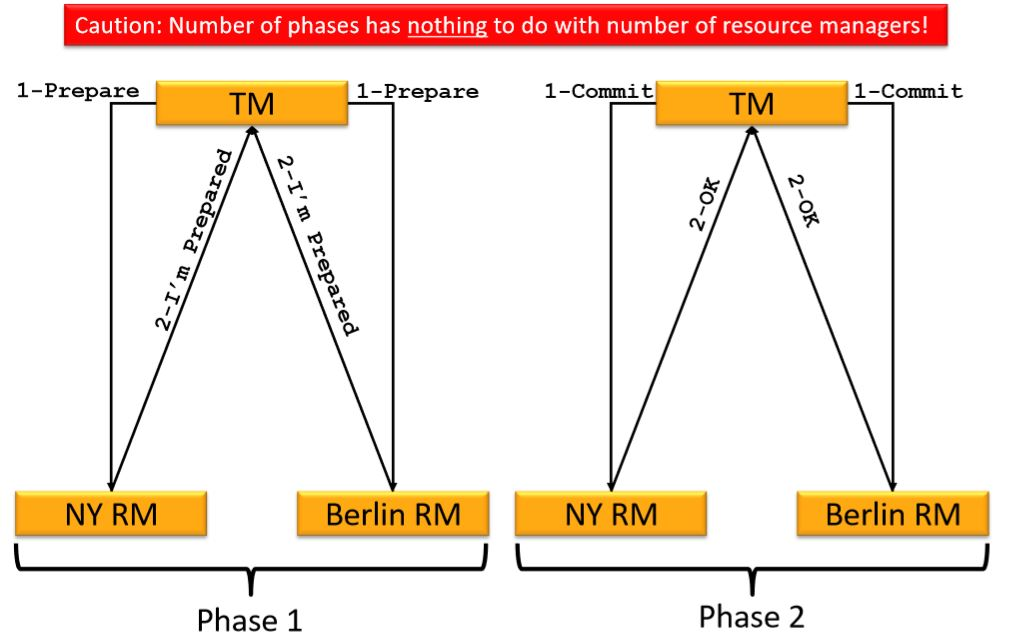
\includegraphics[scale=0.3]{res/two_phase_commit_protocol.jpg}
					\caption{Two Phase Commit Protocol}
				\end{figure}
			
			\subsubsection{Atomic Commitment Protocol (ACP)}
				\begin{itemize}
				 \item All participants that reach a decision reach the same one
				 \item A participant cannot reverse its decision after it has reached one 
				 \item The COMMIT decision can only be reached if all participants voted YES 
				 \item  If all participants voted YES and no failure occurred the decision will finally be COMMIT 
				 \item If all existing failures are repaired and no new failures occurred for sufficiently long, then all participants eventually reach a decision 
			\end{itemize}
			
		\newpage	
		\subsection{Recovery}
			\subsection{2PC Message Flow and Logging}
				\begin{figure}[h!]
					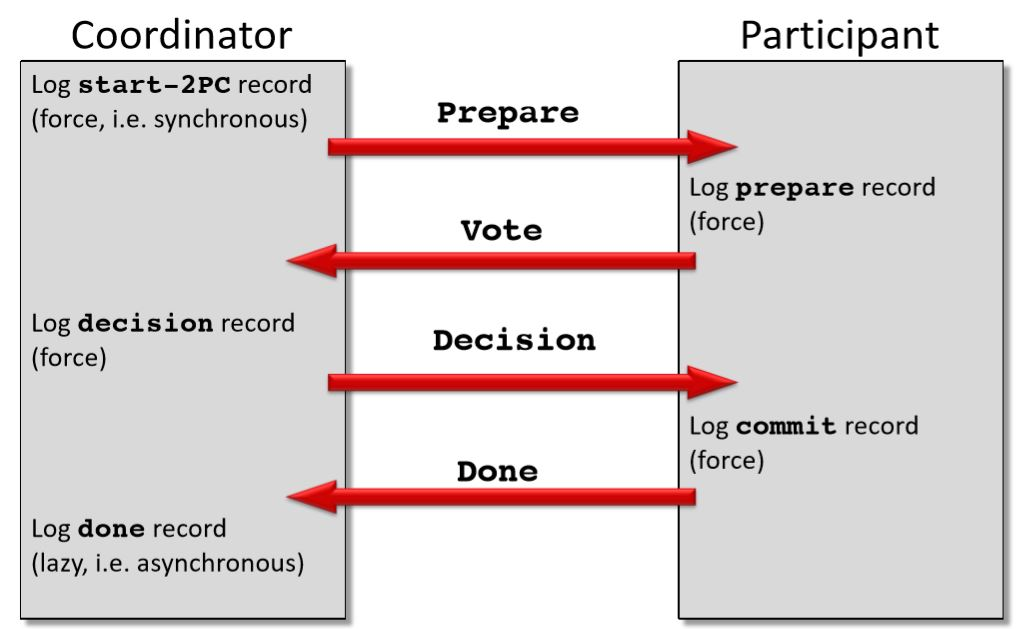
\includegraphics[scale=0.25]{res/message-flow_logging.jpg}
					\caption{Message Flow and Logging}
				\end{figure}
			\subsubsection{Coordinator Recovery}
				\begin{figure}[h!]
					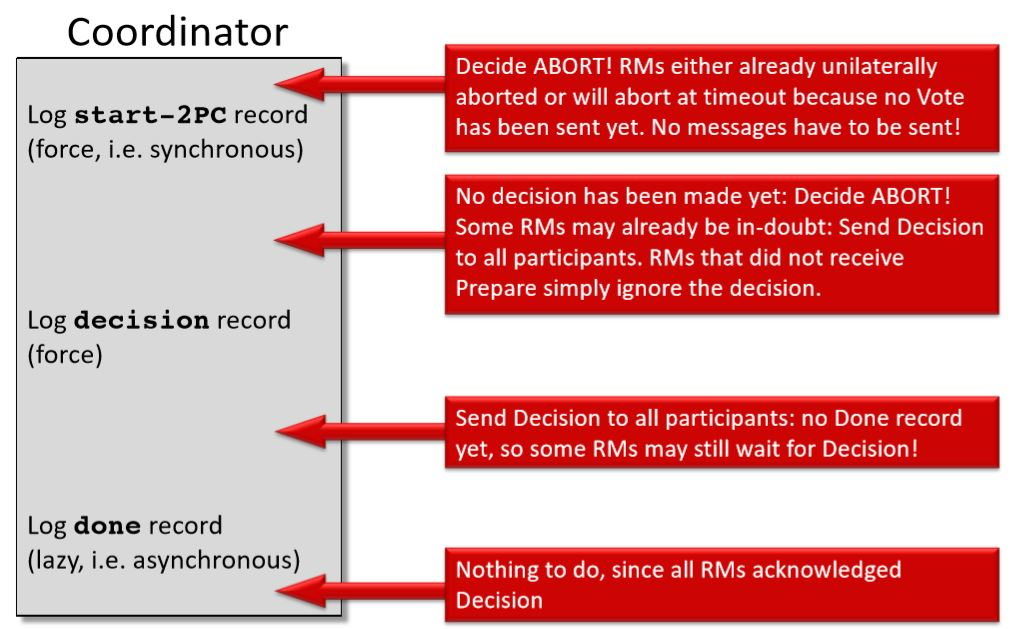
\includegraphics[scale=0.25]{res/coordinator_recovery.jpg}
					\caption{Coordinator Recovery}
				\end{figure}
			\subsubsection{Participant Recovery}
				\begin{figure}[h!]
					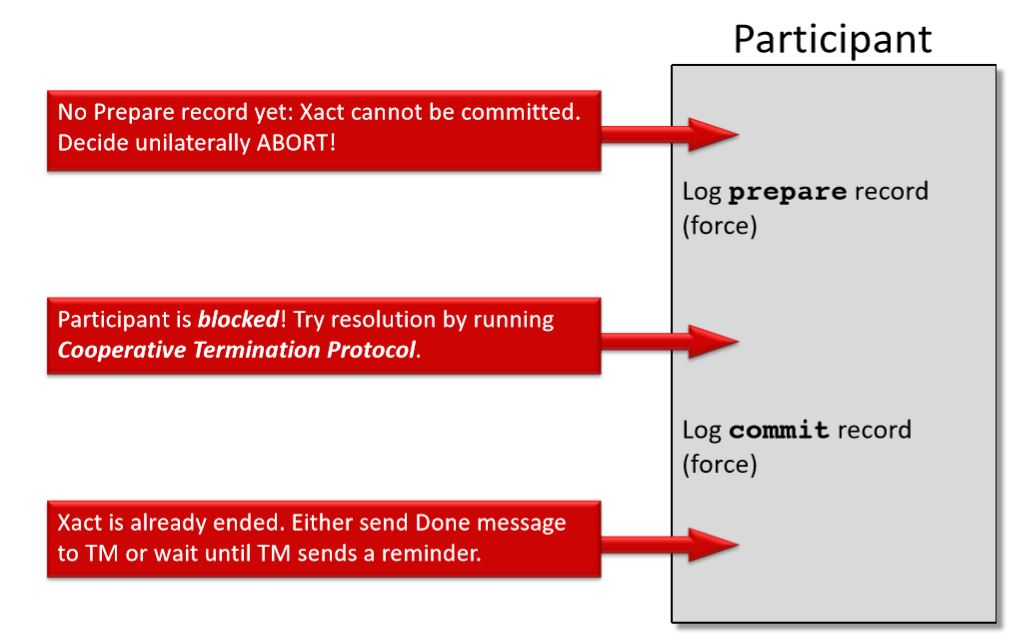
\includegraphics[scale=0.25]{res/participant_recovery.jpg}
					\caption{Participant Recovery}
				\end{figure}
			
		\clearpage	
		\subsection{Blocking Participants}
			\begin{itemize}
				\item During the time interval from having prepared until reception of the TM's decision a participant is blocked ("in-doubt") 
					\subitem \blue{Blocking}:= RM waits for decision message of TM 
					\subitem If TM fails during this period RMs have to wait until TM recovers 
					\subitem If RM fails during this period it must establish connection to TM to recover any in-doubt transaction 
					\subitem Network fragmentation may separate TM from some RMs causing blocking
				\item \blue{Cooperative Termination Protocols}: allow in certain situations to end a transaction without a connection to TM 
				\item  \blue{Heuristic termination}: often used in practice 
					\subitem Blocked RM assumes that its decision is the one of TM too
					
		\end{itemize}
		
		\subsection{Cooperative Termination Protocol}
		
			\begin{itemize}
				\item Together with PREPARE request TM sends list of all participants 
				\item Participants log this list together with VOTE record
				\item  When in-doubt participant ("initiator") cannot connect to TM it contacts reachable participants ("responder") from this list 
					\subitem If all responders are in doubt initiator remains in-doubt too 
					\subitem If at least one responder knows TM's decision (commit or abort) initiator decides accordingly 
					\subitem If at least one responder has not voted yet responder unilaterally decides ABORT and initiator decides accordingly
					
			\end{itemize}
		
		\subsection{Transaction branches}
		
			\begin{itemize}
				\item When an application communicates with another application associated with another transaction manager, a new branchof the same global transaction is created 
					\subitem A.k.a. “transaction infection”
					\subitem This happens based on receiving a transaction context
				\item A resource manager may have more than one active branch for the same global transaction
				\item All branches belong to the same global transaction, i.e. all branches either commit or abort
				
			\end{itemize}
		
			\begin{figure}[h!]
				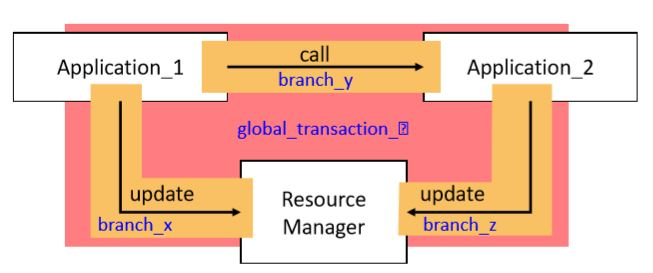
\includegraphics[scale=0.4]{res/transaction_branches.jpg}
				\caption{Transaction Branches}
			\end{figure}
		\pagebreak
		
		
					
			
		
		
		
		
		
		
		
		
		
		
		
			
		